\section{Przypadek Testowy 3 - Algorytm genetyczny - zależność PRD od użytej metody selekcji}
  \subsection{Cel:}
    W tej części zostaną ze sobą porównane PRD rozwiązania algorytmu genetycznego w zależności użytej metody selekcji.
    \subsection{Założenia:}
    Do badania tego przypadku została wykorzystana instancje 
    \begin{itemize}
      \item berlin52.tsp
      \item eil76.tsp
      \item eil51.tsp
      \item gr17.tsp
      \item gr21.tsp
      \item gr24.tsp
      \item gr48.tsp
      \item hk48.tsp
      \item kroA100.tsp
      \item kroA150.tsp
      \item kroB100.tsp
      \item kroB150.tsp
      \item swiss42.tsp
      \item ftv33.atsp
      \item ftv35.atsp
      \item ftv38.atsp
      \item ftv44.atsp
      \item ftv47.atsp
      \item br17.atsp
    \end{itemize}
    Dodatkowo współczynnik mutacji został ustalony na 0.2, liczba iteracji została ustalona na 200, wielkość populacji została ustalona na 100. współczynnik selekcji był w zakresie \(SR \in {0.5, 0.55, 0.6 ... 0.9}\).
    \subsection{Metody selekcji:}
    \subsubsection{Ruletka:}
    Metoda selekcji przedstawicieli populacji polega na znormalizowaniu współczynnika dopasowania tak że suma wszystkich wynosi 1 odwrotnie proporcjonalnie do długości ścieżki. Następnie losowana jest liczba z przedziału \( [0, 1)\). Do nowej populacji dopisywana jest jedna ścieżka aż nowa populacja będzie tego samego rozmiaru co poprzednia.
    \subsubsection{Odcięcie:}
    Metoda selekcji przedstawicieli populacji polega na posortowaniu populacji względem długości rozwiązania i odcięcie sparametryzowanej najgorszej części (np. 10\%). aby uzupełnić populację najlepsze odobniki są doklejane po raz kolejny.
  \subsection{Wyniki: }
  Poniższa tabela przedstawia wyniki testów, odchylenie standardowe oraz błęd standardowy.
  \begin{table}[!ht]
    \centering
    \begin{tabular}{|l|l|l|l|l|l|l|l|l|l|}
    \hline
        SR & O & R & T & SD\textsubscript{O} & SD\textsubscript{R} & SD\textsubscript{T} & SE\textsubscript{O} & SD\textsubscript{R} & SD\textsubscript{T} \\ \hline
        0.5 & 90.31 & 274.21 & 76.47 & 104.79 & 207.25 & 84.46 & 24.70 & 48.85 & 19.91 \\ \hline
        0.55 & 85.55 & 270.70 & 67.55 & 100.87 & 208.68 & 81.11 & 23.77 & 49.19 & 19.12 \\ \hline
        0.6 & 86.40 & 271.83 & 74.78 & 100.70 & 210.56 & 83.83 & 23.74 & 49.63 & 19.76 \\ \hline
        0.65 & 87.69 & 269.76 & 71.43 & 103.10 & 211.25 & 83.36 & 24.30 & 49.79 & 19.65 \\ \hline
        0.7 & 91.79 & 272.51 & 75.35 & 106.24 & 205.00 & 84.03 & 25.04 & 48.32 & 19.81 \\ \hline
        0.75 & 91.51 & 273.32 & 74.74 & 108.68 & 216.22 & 85.11 & 25.62 & 50.96 & 20.06 \\ \hline
        0.8 & 93.19 & 264.47 & 71.91 & 105.50 & 204.03 & 87.26 & 24.87 & 48.09 & 20.57 \\ \hline
        0.85 & 91.89 & 272.87 & 79.23 & 108.05 & 207.47 & 86.79 & 25.47 & 48.90 & 20.46 \\ \hline
        0.9 & 98.22 & 262.21 & 72.88 & 117.56 & 185.75 & 83.56 & 27.71 & 43.78 & 19.69 \\ \hline
        0.95 & 113.79 & 263.77 & 71.11 & 120.98 & 199.82 & 82.98 & 28.52 & 47.10 & 19.56 \\ \hline
    \end{tabular}
    \caption{
      SR - współczynnik selecji,
      O - PRD dla selekcji przez odcięcie, 
      R - PRD dla selekcji przez ruletkę, 
      T - PRD dla selekcji przez turniej, 
      SD\textsubscript{O} - odchylenie standardowe dla selekcji przez odcięcie, 
      SD\textsubscript{R} - odchylenie standardowe dla selekcji przez ruletkę, 
      SD\textsubscript{T} - odchylenie standardowe dla selekcji przez turniej, 
      SE\textsubscript{O} - Błąd standardowy dla selekcji przez odcięcie,
      SE\textsubscript{R} - Błąd standardowy dla selekcji przez ruletkę, 
      SE\textsubscript{T} - Błąd standardowy dla selekcji przez turniej
    }

  \end{table}
    Odchylenie standardowe oraz błąd standardowy zostały obliczone według wzorów: \\
    Odchylenie standardowe:
    \[ \sigma = \sqrt{\frac{\sum_{n = 1}^{18}(\bar{x} - x_n)^2}{18}} \]
    Błąd standardowe:
    \[ \sigma_{\bar{x}} = \frac{\sigma}{\sqrt{18}} \]

  \subsection{Wykresy: }
    \begin{figure}[H]
      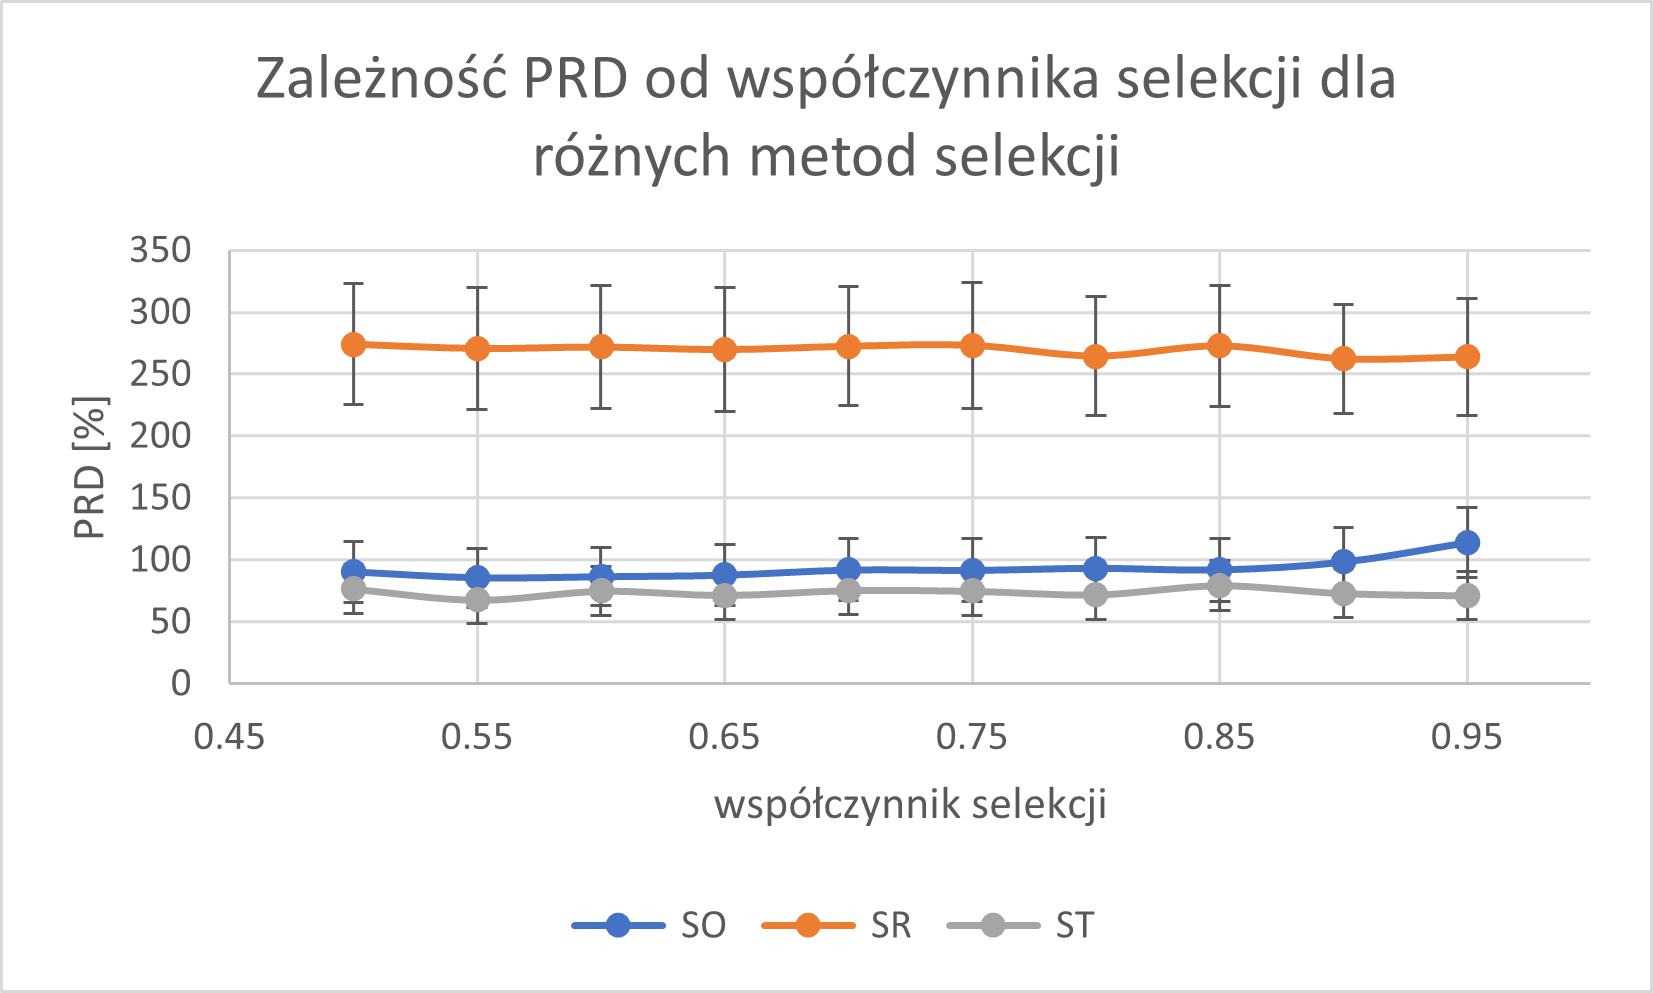
\includegraphics[scale=0.9]{chart_test_3.png}
      \centering
      \caption{zależność PRD od współczynnika selekcji}
    \end{figure}
  
    Na wykresach przedstawione są średnie wartości PRD dla badanych danych.
  \subsection{Wnioski: }
  Selekcja przez odcięcie oraz turniejowa sprawdza się zdecydowanie lepiej niż selekcja metodą ruletki. W metodzie ruletki najsłabsze osobniki mają szansę przejść do krzyżowania gdzie w metodzie odcięcia oraz w turnieju są zawsze usuwane i krzyżują się tylko najlepsze cechy.
